\section{Diskussion}
\label{sec:Diskussion}

\section{Diskussion}
Aus \autoref{fig:1} lässt sich erkennen, dass die Strömungsgeschwindigkeit $v$ linear von der Frequenzverschiebung durch den Cosinus des Dopplerwinkels $\frac{\Delta\nu}{\cos{\alpha}}$ abhängt. Daraus folgt, dass bei kleineren Geschwindigkeiten die Frequenzen weniger verschoben werden, was den Doppler-Effekt bestätigt.\\
In den Strömungsprofilen aus \autoref{fig:2} und \autoref{fig:3} zeigen die Geschwindigkeiten und Streuintensitäten parabelförmige Muster. Bei nicht so hohen Geschwindigkeiten bewegen sich die Parabeln gespiegelt, wie bei \autoref{fig:2}, wohingegen bei höheren Geschwindigkeiten die Frequenzen weiter verschoben werden, sodass ein fast ähnlich orientiertes Profil, wie bei \autoref{fig:3} entstehen kann. Daraus lässt sich erkennen, dass es sich um ein laminares Strömungsprofil handeln muss.

\section{Anhang}
\begin{figure}[H]
  \centering
  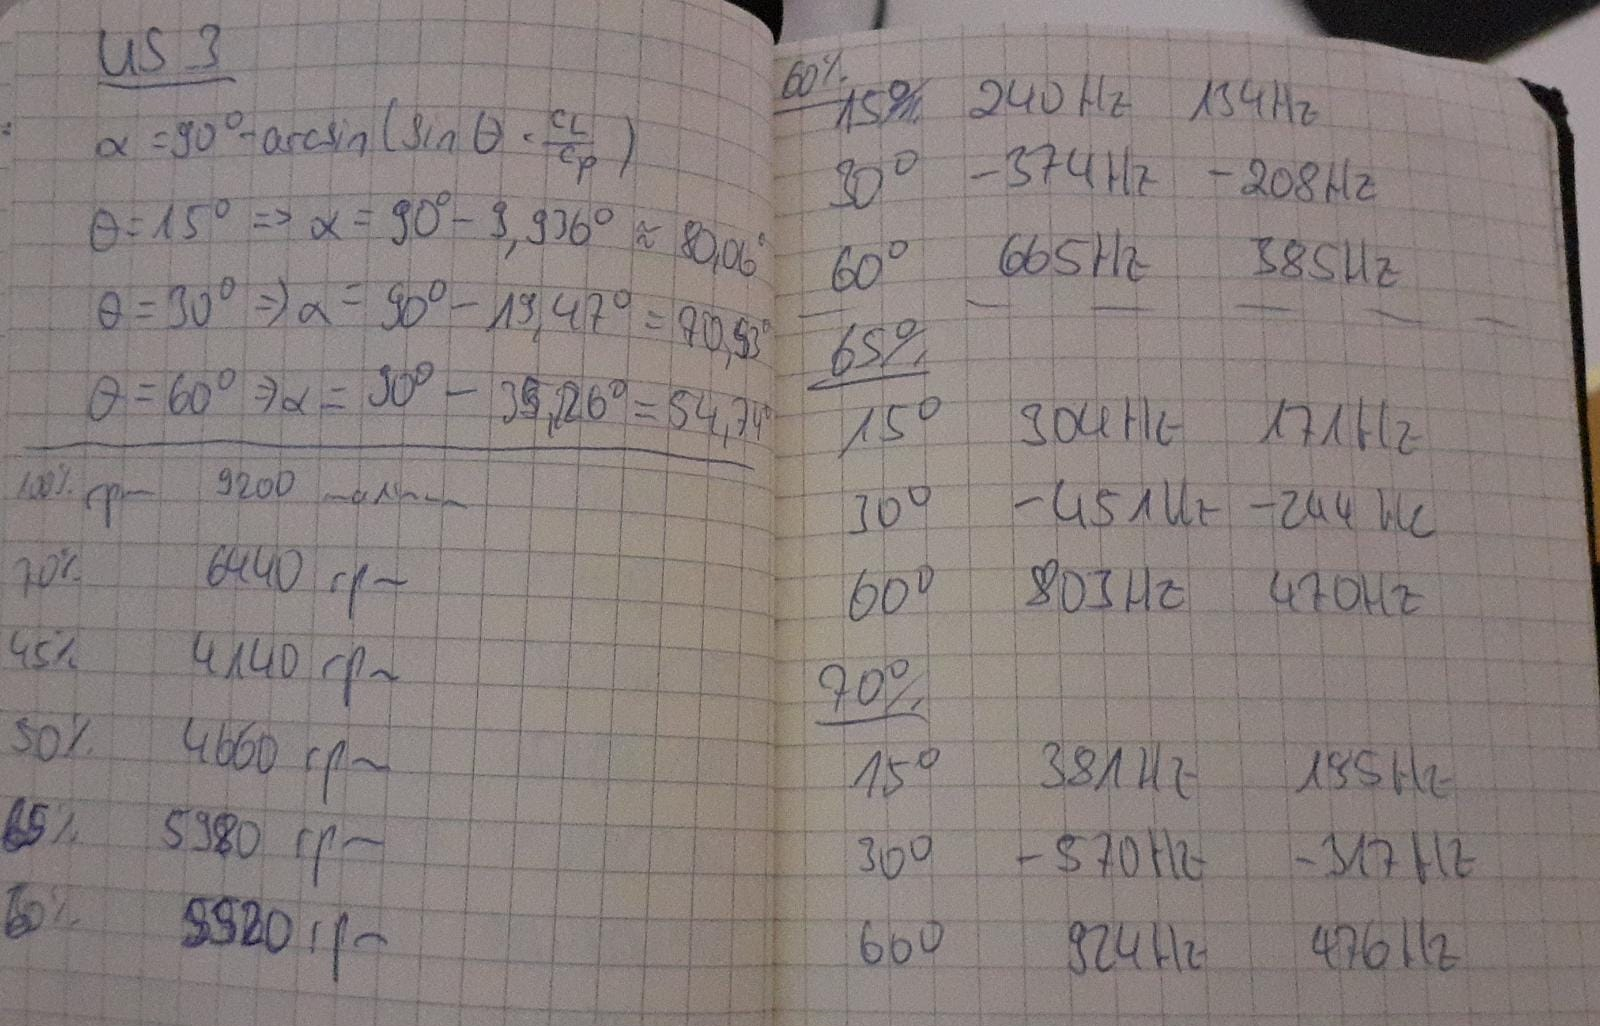
\includegraphics[width=9cm]{content/a1}
  \caption{Originale Messdaten.}
\end{figure}
\begin{figure}[H]
  \centering
  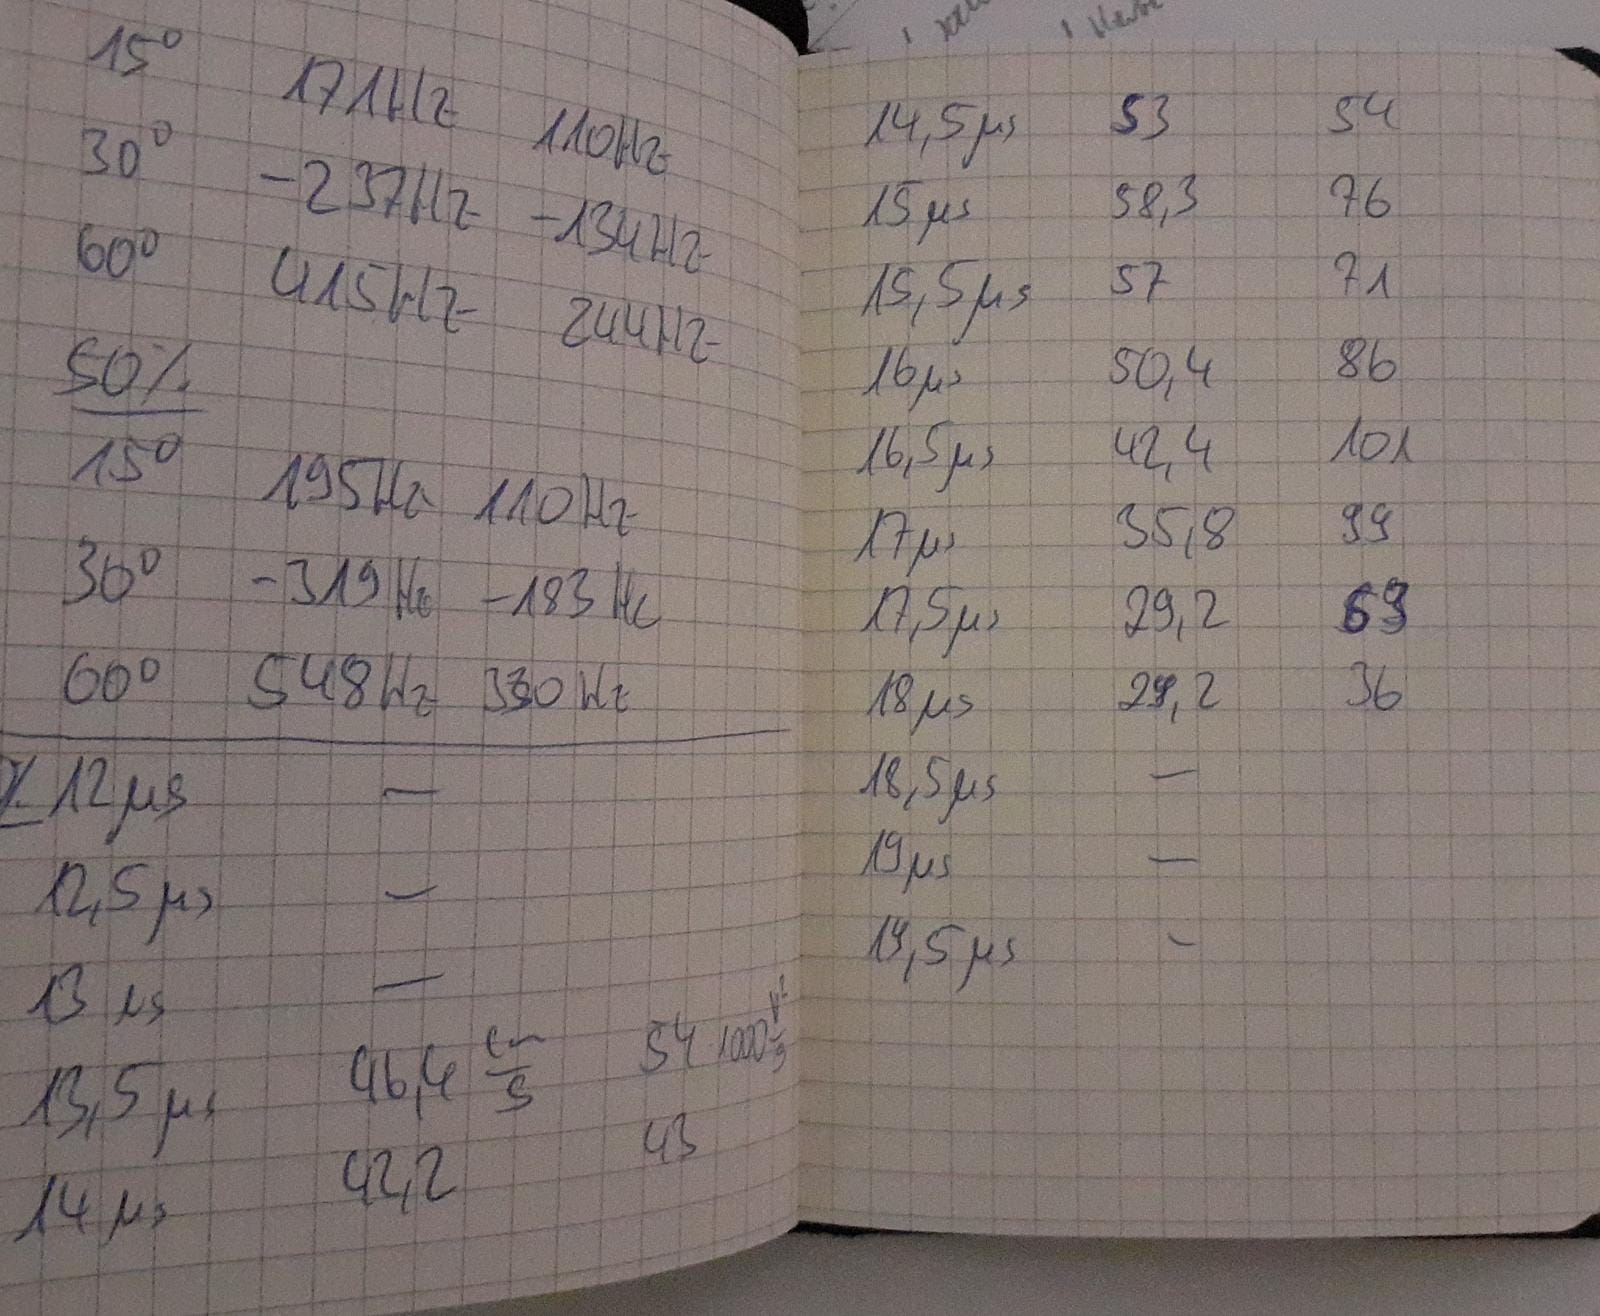
\includegraphics[width=9cm]{content/a2}
  \caption{Originale Messdaten.}
\end{figure}
\begin{figure}[H]
  \centering
  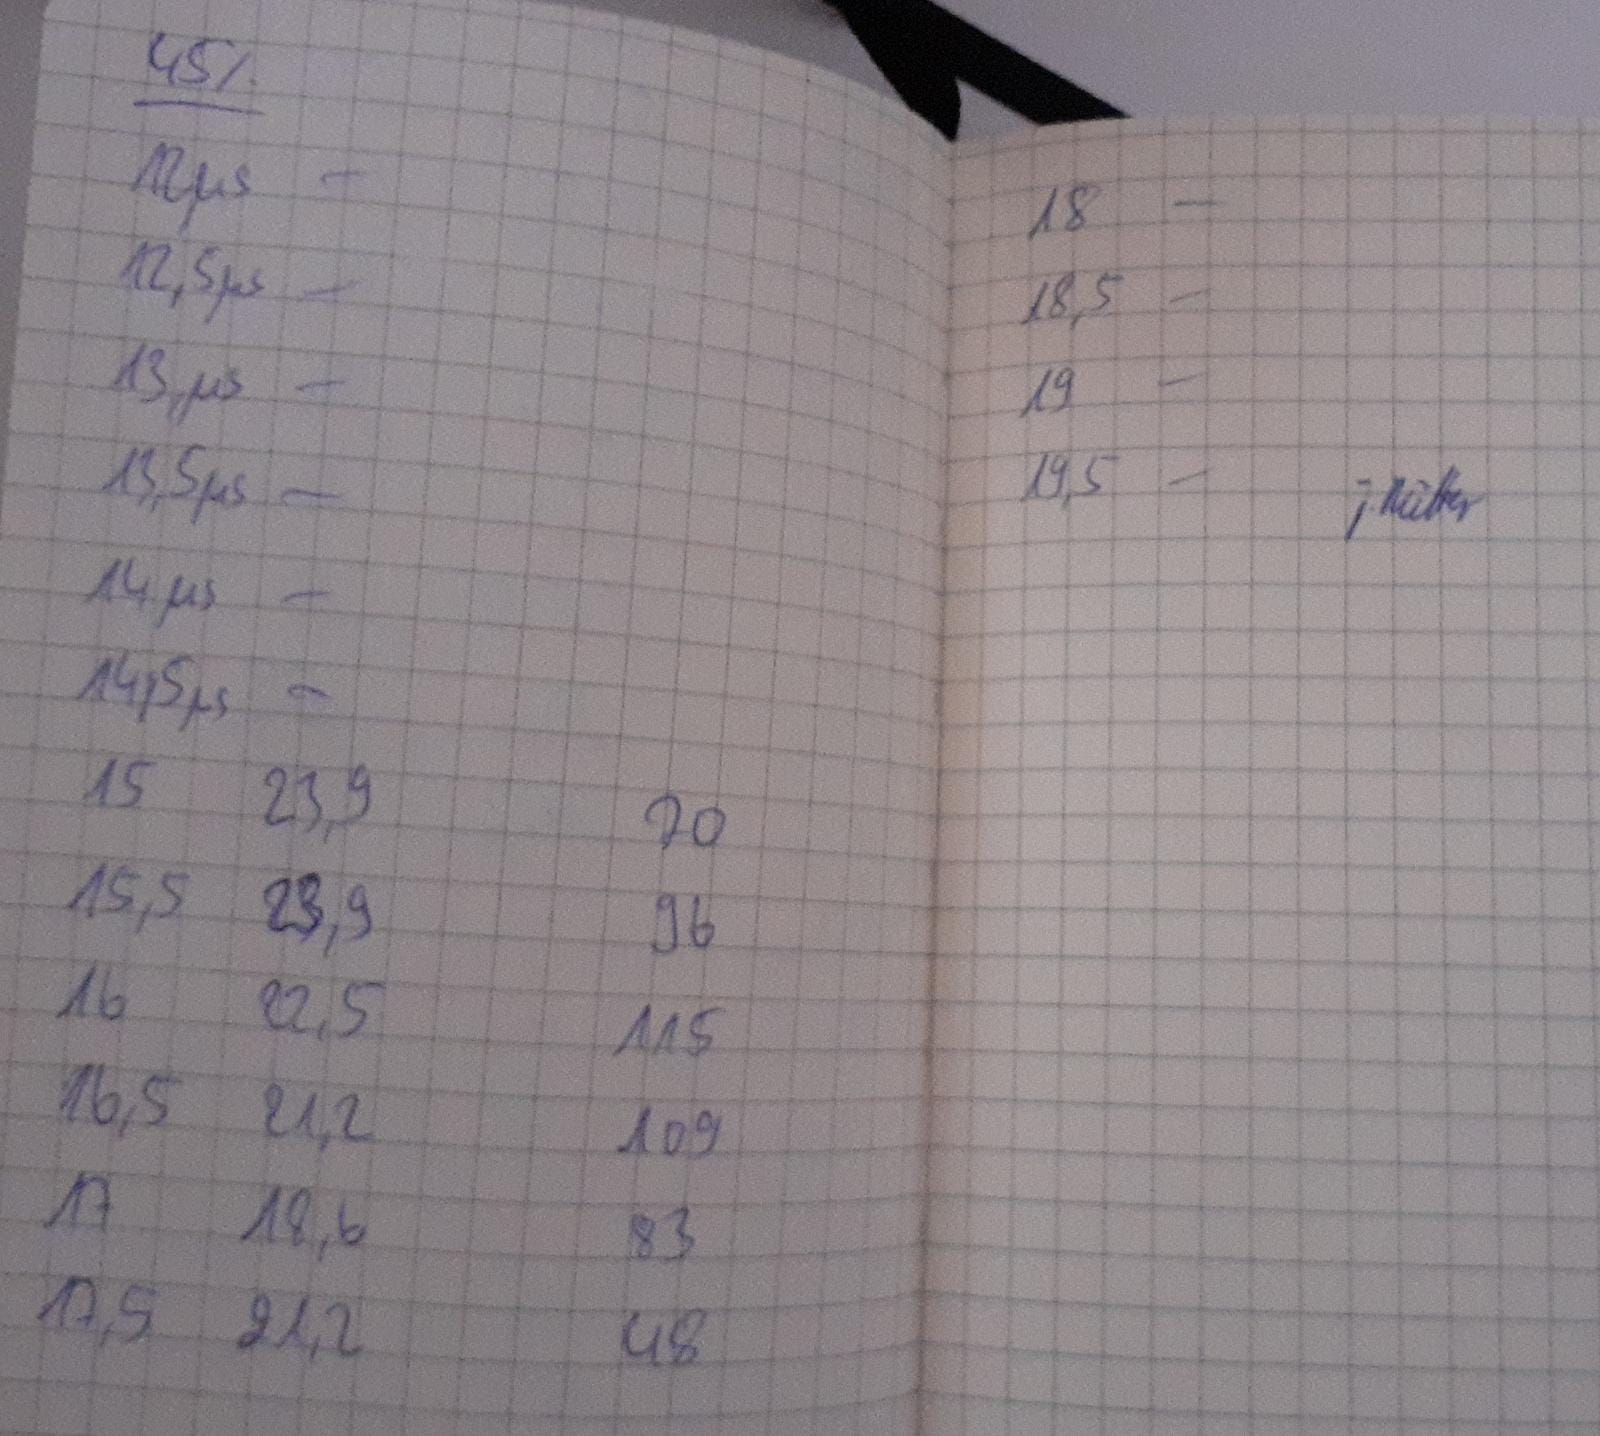
\includegraphics[width=9cm]{content/a3}
  \caption{Originale Messdaten.}
\end{figure}
